% -*-LaTeX-*-

\documentclass[12pt]{article}

\newif\ifHtml
\Htmlfalse

\newif\ifPDF
\PDFtrue

\ifHtml
  \PDFfalse
  \usepackage[tex4ht,colorlinks=true,linkcolor=blue,citecolor=blue,urlcolor=blue,pdftitle={Signal Computing: Digital Signals in the Software Domain}]{hyperref}
  \hyperlinkfileprefix{}
\else
  \ifPDF
    \usepackage[pdftex,pdftitle={Signal Computing: Digital Signals in the Software Domain},colorlinks=true,linkcolor=blue,citecolor=blue,urlcolor=blue,bookmarks,bookmarksopen]{hyperref}
    \usepackage{fullpage}
  \else
    \usepackage{hyperref}
    \usepackage{mathptmx,helvet,courier,fullpage}
  \fi
\fi


\usepackage{fullpage,graphicx,algorithmic,multirow,rotating}
\usepackage[T1]{fontenc}
%\usepackage{listings}
\usepackage{matlab-prettifier}

%\usepackage{html}
%\usepackage{algorithm}
\usepackage{titlesec}
\newcommand{\sectionbreak}{\clearpage}
\usepackage{chngcntr}
\counterwithin{figure}{section}

% Superscripts outside math mode
\newcommand{\spscript}[2]{\mbox{#1}$^\mathrm{#2}$}

\renewcommand{\textfraction}{0.05}
\renewcommand{\floatpagefraction}{0.9}
\newcommand{\block}[1]{\textbf{\itshape #1}}
\newcommand{\menu}[1]{\textbf{#1}}
\newcommand{\button}[1]{[#1]}
\newcommand{\option}[1]{``#1''}

% XMP include for Creative Commons
\usepackage{xmpincl}
\includexmp{metadata}

% Fancy page headings
\usepackage{fancyhdr}
\setlength{\headheight}{15pt}

\fancyhf{} % clear all header and footer fields
\fancyfoot[L]{Signal Computing}
\fancyfoot[R]{Laboratory Manual}
\fancyhead[L]{\slshape\leftmark}
\fancyhead[R]{\thepage}
\renewcommand{\headrulewidth}{0.4pt}
\renewcommand{\footrulewidth}{0.4pt}

\fancypagestyle{plain}{%
\fancyhf{} % clear all header and footer fields
\fancyfoot[L]{Signal Computing}
\fancyfoot[R]{Laboratory Manual}
\fancyhead[R]{\thepage}
\renewcommand{\headrulewidth}{0pt}
\renewcommand{\footrulewidth}{0.4pt}}

\pagestyle{fancy}

% Math and logic
\usepackage{amsmath}
\usepackage{mathtools}
\newcommand{\pred}[1]{\ensuremath{\textit{#1}}}
\newcommand{\const}[1]{\ensuremath{\textsf{#1}}}
\newcommand{\deriv}[2]{\ensuremath{\frac{\mathrm{d} #1}{\mathrm{d} #2}}}
\newcommand{\derivin}[2]{\ensuremath{{\mathrm{d} #1}/{\mathrm{d} #2}}}
\newcommand{\sderiv}[2]{\ensuremath{\frac{\mathrm{d}^{2} #1}{\mathrm{d} #2^{2}}}}
\newcommand{\nderiv}[3]{\ensuremath{\frac{d^{#3} #1}{d #2^{#3}}}}
\newcommand{\pderiv}[2]{\ensuremath{\frac{\partial #1}{\partial #2}}}
\newcommand{\spderiv}[2]{\ensuremath{\frac{\partial^2 #1}{\partial #2^{2}}}}
\newcommand{\pderivin}[2]{\ensuremath{{\partial #1}/{\partial #2}}}
\newcommand{\spderivin}[2]{\ensuremath{{\partial^2 #1}/{\partial #2^{2}}}}
\newcommand{\transpose}{\ensuremath{^{\mathsf{T}}}}
\DeclareMathOperator{\Real}{Re}
\DeclareMathOperator{\Imag}{Im}
\DeclareMathOperator{\sinc}{sinc}

\newcommand{\commentedout}[1]{}

\title{Signal Computing: Digital Signals in the Software
  Domain\\[2\parskip]
Laboratory Manual}

\author{Michael Stiber \and Bilin Stiber \and Eric C. Larson}

% \date{August 2014}

\begin{document}
\lstset{style=Matlab-editor}
\lstset{basicstyle=\mlttfamily}

\begin{titlepage}

\mbox{}\\[0.5in]
\begin{center}
\mbox{}\hrulefill\mbox{}\\[0.25in]
{\Huge Signal Computing:}\\[0.25in]
{\LARGE Digital Signals in the Software Domain}\\[0.25in]
\mbox{}\hrulefill\mbox{}\\[0.5in]
{\Huge Laboratory Manual: Matlab Edition}\\[2.5in]

\mbox{}\hfill
\parbox{1.5in}{\mbox{}}
\parbox{3in}{Fall 2016}\\[0.25in]
\mbox{}\hfill
\parbox{3in}{\raggedright
Michael Stiber\\
Bilin Zhang Stiber\\
University of Washington Bothell\\
18115 Campus Way NE\\
Bothell, Washington 98011\\[0.25in]
Eric C. Larson\\
Southern Methodist University\\
Lyle School of Engineering\\
3145 Dyer Street\\
Dallas, TX 75205}
\end{center}

\newpage
\mbox{}\vspace{4in}
\begin{flushright}
Copyright \copyright\ 2002--2016 by Michael and Bilin Stiber and Eric
C. Larson\\[2in]
This work is licensed under the Creative Commons
Attribution-ShareAlike 4.0 International License. To view a copy of
this license, visit
\url{http://creativecommons.org/licenses/by-sa/4.0/}.\\
\includegraphics[height=1.5in]{by-sa}
\end{flushright}

\thispagestyle{empty}

\end{titlepage}

\tableofcontents

%&LaTeX

\section{The Matlab Lab, or How Not to Teach a Programming Language}

Labs in this class will make liberal use of the Matlab numerical
programming environment. Because this class assumes that you are an
experienced computer science student, you are expected to be able to
learn how to use computer tools, and how to program in new programming
languages, pretty much on your own. So, the first thing you should do
is check out the Matlab documentation built into the Matlab help
system, or online at
\url{http://www.mathworks.com/help/matlab/index.html}. Of course, you
can always search online for Matlab tutorials and the like. We'll
include a very brief overview of Matlab below, and then more detailed
information about the code developed specifically for this class that
you will be using.

\section{Matlab in a (Very Small) Nutshell}
\label{sc:basic-matlab}

The Matlab GUI environment is very similar to IDEs that you are
already familiar with. As you might expect, there are some
idiosyncrasies here and there, but nothing terribly unexpected. The
major areas of difference are tools and panes that have to do with
viewing variables (something in other IDEs that you'd only see when
debugging a program), the command pane, and figure windows that open
to display graphs. The first two of these differences have to do with
the fact that Matlab is an interpreted language/programming
environment. You primary area of interaction with the Matlab
interpreter will be through the command window, with variable
information panes providing views of variables and their contents
related to your interaction. It's interesting to note that, if you
want, you can run Matlab without the GUI, providing just a command
line interface.

Interpreted languages have their advantages and disadvantages.  One
advantage is that anything you can use as a line of code in a program
you can use immediately as a command on the command line. This lets
you test code interactively and then copy it into the script or
function you're writing. Like any IDE, Matlab includes an editor with
syntax highlighting and debugger integration.

The disadvantage is the interpreted programs are slower. In Matlab, we
get around this by using built-in functions that operate on entire
vectors or arrays as single data objects. The core loops of the
built-in functions are compiled for speed. If you make good use of
those functions, Matlab code can often be as fast as completely
compiled code.

Here are some things to try:
\begin{enumerate}
\item Immediate calculations and variables:
\begin{verbatim}
   radius = 5    % Comments start with "%"
   circumference = 2 * pi * radius
   area = pi * radius^2
\end{verbatim}
\item Complex numbers:
\begin{verbatim}
   sqrt(-1)
   x = 7 + 14j
   conj(x)       % complex conjugate
   abs(x)        % magnitude (e.g., for polar representation)
   angle(x)      % and angle for polar rep
   real(x)
   imag(x)
\end{verbatim}
\item Complex exponentials:
\begin{verbatim}
   exp(j * pi)
   exp(j * pi/2)
   exp(j * pi/4)
\end{verbatim}
\item Vectors:
\begin{verbatim}
   v1 = [0 1 2 3]    % Four elements
   v2 = [0 : 2 : 10] % like a loop (start value : increment : end value)
   v3 = pi * [-0.5 -0.25 0 0.25 0.5] % All operations are vectorized
   exp(j * v3)
   mistake = v1 * v1     % a mistake; vector mult doesn't work this way
   dotproduct = v1 * v1' % transposing will work, if you want to do this
   arrayprod = v1 .* v1  % element-by-element ops include: .+, .-, .*, ./
\end{verbatim}
\item Simple plots (note that ``;'' suppresses outputting results to
  the command window --- useful if that would generate massive amounts
  of text, or just if you want things neat):
\label{it:simple-plots}
\begin{verbatim}
   t = [0 : 0.01 : 2*pi];
   x = sin(t);
   plot(t, x);       % default plots points connected by lines in blue
   plot(t, x, 'r');  % change the line color
   plot(t, x, 'r.'); % change the plot style; zoom in to see individual points
   xlabel('t, ms');  % X axis label (all of your plots should have this)
   ylabel('Mag');    % Y axis label (all of your plots should have this)
   title('Triangle');% Graph title (all of your plots should have this)
\end{verbatim}
\end{enumerate}

If you take a sequence of commands and save them in a file with an
extension of \texttt{.m}, the result is a \emph{script}. Assuming that the
script is saved in a directory in the MATLAB search path, you can then
execute the script by just typing its name (without the \texttt{.m}),
just as if it were a command. If you want your code to take
parameters, return a return value, and have local variables, start
your code with a line like:
\begin{verbatim}
   function retval = funcname(parm1, parm2)
\end{verbatim}
Your code is now a function. MATLAB functions can take variable
numbers of arguments and even return variable numbers of return
values, but that's getting beyond what we need right now.

\paragraph{Step 1.1} Extracting and/or inserting numbers in a
vector is very easy to do. Consider the following definition:
\begin{verbatim}
   x = [ ones(1,4), [2:2:11], zeros(1,3) ]
   x(3:7)
   length(x)
   x(2:2:length(x))
\end{verbatim}
Explain the result echoed from the last three lines of the above code.

\paragraph{Step 1.2} In the previous step, the vector \texttt{x}
contained 12 elements. Observe the result of the following assignment:
\begin{verbatim}
   x(3:7) = pi*(1:5)
\end{verbatim}
Now write a statement that will replace the odd-indexed elements of
\texttt{x} with the constant -77 (i.e., \texttt{x(1)},
\texttt{x(3)}, etc). Use vector indexing and vector replacement.

\ifanswers
\textit{Answer:} \texttt{xx(1:2:length(xx)) = -77}. MATLAB allows
assignment of a scalar to a vector; each element of the vector gets
the same value. Note that you can write this more simply as:
\begin{verbatim}
   xx(1:2:end) = -77
\end{verbatim}
  The keyword \texttt{end}, in this context, indicates the final
  index. It has some other meanings in other contexts; type
  \texttt{help end} to find out about them.
\fi

\paragraph{Step 1.3} Vectorization is an essential programming
skill in Matlab. Loops can be done in Matlab, but they are not the
most efficient way to get things done. It's better to avoid loops and
use the vector notation instead. For example, the code below uses a
loop to compute values of the sine function. Rewrite this computation
without using the loop (as in list item~\ref{it:simple-plots} in
this section).
\begin{verbatim}
   x = [ ];                  % initialize the x vector to a null
   for k=0:7,
      x(k+1) = sin( k*pi/4 ) % x(0) would fail
   end
x
\end{verbatim}

While thinking this way isn't essential in this course (the loop will
still get the job done), it's probably a valuable skill to learn, as
software moves more and more towards taking advantage of multiple
processors. In this case, \texttt{[0:7]} creates a vector of the
values we want, the scalar multiplication \texttt{*pi/4} generates the
vector of inputs for the \texttt{sin()} function, and the function
itself is vectorized (can take a vector as an input argument) and
returns an equal-sized vector of its results, which are in turn
assigned to \texttt{x}.}

\paragraph{Step 1.4} Consider the following code that plots a
sinusoid:
\begin{verbatim}
   t = [0 : 0.01 : 1]; % time in seconds
   f = 5;              % freq in Hertz
   x = sin(2*pi*f*t);
   plot(t, x);
   xlabel('Time (sec)');
\end{verbatim}
Use the MATLAB editor to create a script file called
\texttt{firstsin.m}, verify that you've saved it in a directory in the
MATLAB path (or add that directory to the path), and test its
execution by typing \texttt{firstsin} at the MATLAB command
prompt. Note that you can also do:
\begin{verbatim}
   type firstsin   % prints out contents of the script
   which firstsin  % shows directory (useful when your code shadows built-ins)
\end{verbatim}

Add three lines of code to your script, so that it will plot a cosine
on top of the sine in a different color. Use the \texttt{hold}
function to add a plot of
\begin{verbatim}
   0.5*cos(2*pi*f*t)
\end{verbatim}
to the plot. See \texttt{help hold} in MATLAB. Enter the three lines
of code you added below. Save the plot using the MATLAB \texttt{print}
command as a JPEG file named \texttt{step14.jpg} by typing:
\begin{verbatim}
   print -djpeg step14
\end{verbatim}
You should include all plots in your lab report, following the
instructions in the report rubric.

\ifanswers
\textit{Answer:} The three lines of code should be something like:
\begin{verbatim}
   hold on;           % so that the new plot goes on top of the old
   y = 0.5*cos(2*pi*f*t);
   plot(t, y, 'r');   % Should add a new plot
\end{verbatim}
\fi

\paragraph{Step 1.5} Now generate a tone (i.e., a sinusoid) in MATLAB
and listen to it with the \texttt{sound} command. The frequency of
your tone should be 2 kHz and the duration should be 1 sec. The
following lines of code should be saved in a file called
\texttt{mysound.m} and run from the command line:
\begin{verbatim}
   dur = 1.0;
   f = 2000;
   fs = 8000;
   t = [0 : (1/fs) : dur];
   x = sin(2*pi*f*t);
   sound(x, fs)
\end{verbatim}
The sound hardware will convert the vector of numbers \texttt{x} into
a sound waveform at a certain rate, called the sampling rate (we will
learn a lot more about this in this class). In this case, the sampling
rate is 8000 samples/second, but other values might be used depending
on the capability of sound hardware. What is the length of the vector
\texttt{x}?

\paragraph{Step 1.6} Write a new function that performs the same task
as the following function without using a \texttt{for} loop. Use the
idea in step~1.3 and also consult the section on vector logicals in
the MATLAB documentation. In addition, the MATLAB logical operators
are summarized via \texttt{help relop}.
\begin{verbatim}
   function Z = replacez(A)
   %REPLACEZ Function that replaces the negative elements
   % of a matrix with the number 77
   % usage:
   % Z = replacez(A)
   % A = input matrix whose negative elements are to
   % be replaced with 77
   %
   [M,N] = size(A);
   for i=1:M
      for j=1:N
         if A(i,j) < 0
            Z(i,j) = 77;
         else
            Z(i,j) = A(i,j);
         end
      end
   end
\end{verbatim}

\ifanswers
\textit{Answer:} Here's an example without the \texttt{for} loops (comments
  eliminated for brevity's sake):
\begin{verbatim}
   function Z = replacez(A)
   Z = A;
   Z(Z<0) = 77;
   % Note: Z = (A .* (A>=0) + 77 .* (A<0)); would also work
\end{verbatim}
\fi


\subsection{Representing Analog, Discrete, and Digital Signals}

In our class, we will need to manipulate analog signals (real-valued
signals that are functions of continuous time), discrete signals
(real-valued signals that are functions of discrete time), and digital
signals (discrete-valued signals that are functions of discrete
time). No need to worry about the details or these; that will become
clear later. The trickiest part of this is representing anything other
than digital signals on a digital computer, because you can't. So,
we'll need to employ two key elements of software design: information
hiding and make-believe.

\begin{figure}
\begin{center}
\includegraphics[width=0.75\textwidth]{lab1/AnalogSignal-help}
\end{center}
\caption{.\label{fg:analogsignal-help}}
\end{figure}

Information hiding is used in our implementation of analog signals. We
make use of the object-oriented programming aspects of Matlab to
create an \texttt{AnalogSignal} class. If you look up the documentation
for \texttt{AnalogSignal} (using \texttt{doc AnalogSignal}), you'll
see something like figure~\ref{fg:analogsignal-help}. The key
operations on these analog signals are:
\begin{itemize}
\item Creating an analog signal (ex: \texttt{a =
    AnalogSignal('sawtooth', 2.0, 1.0, 10.0)}).
\item Scaling an analog signal (ex: \texttt{b = a * 5})
\item Adding two analog signals (ex: \texttt{c = a + b})
\item Subtracting two analog signals (ex: \texttt{d = c - a})
\item Plotting an analog signal (ex: \texttt{plot(d)})
\item Sampling an analog signal (ex: texttt{x = d.samplehold(0.1)})
\end{itemize}

You will get a lot more experience working with analog signals shortly
in this class, so for the time being just play with this a bit.



%&LaTeX

\section{Let's Get Digital}

In this lab, you will use Matlab to explore how a physical signal can
be considered to be composed of a sum of sinusoids --- its
\emph{Fourier series}. You will then investigate how capturing this
signal for computer use --- sampling and quantization --- modifies the
signal. Finally, you will see how the choices you make in the
parameters for sampling and quantization affect the quality of the
digitized, computer signal. You will be using the Matlab
\texttt{AnalogSignal} class and functions at
\url{http://faculty.washington.edu/stiber/pubs/Signal-Computing/}.

\subsection{Fourier series representation of a physical signal}

In this section, you will use the Matlab \texttt{AnalogSignal} class
to simulate an analog signal generator. The constructor takes the
following arguments:
\begin{verbatim}
% AnalogSignal(type, amplitude, frequency, dur)
%    Where:
%    type = 'sine', 'cosine', 'square', 'sawtooth', or 'triangle'
%    amplitude = signal amplitude
%    frequency = signal frequency
%    dur = signal duration
\end{verbatim}

Remember that, though an \texttt{AnalogSignal} is simulating an analog
signal, in Matlab all functions are sampled at discrete points in
time. The crufty details of this are hidden away in the class's
implementation.

\paragraph{Step 1.1} Verify that you can get a triangle wave. What is
the code to generate and plot a triangle wave ranging from -1 to 1
Volts with a frequency of 10Hz and a duration of 1sec?

\paragraph{Step 1.2} Recall that any periodic signal can be
represented as a sum of harmonic sinusoids.  The amplitude of each
harmonic is known as the Fourier Series. It may at first seem like
sums of sinusoids would be poor approximations of real periodic
signals, but this is not the case. We can illustrate this using a
triangle wave. The formula for synthesis of a triangle wave with
frequency $\omega_0$ is a sum of harmonically related sine waves (its
Fourier series):
  \[
  x(t) = \sum_{k=0}^{\infty}
  \left( 
    \underbrace{ \frac{8}{\pi^2} \frac{(-1)^k}{(2k+ 1)^2} }_{ \text{amplitude} } 
    \underbrace{ \sin((2k+1)\omega_0 t) }_{ (2k+1)^{th}\text{ harmonic} } 
  \right)
  \]
  In this case, in the analog domain, we are dealing with frequencies
  in Hz, and so $\omega_0 = 2\pi f_0$. Notice that the Fourier Series
  of the triangle wave only uses odd harmonics (i.e., the only
  non-zero frequencies are $(2k+1)\omega_0=\omega_0, 3\omega_0,
  5\omega_0 \cdots$). Also notice that resulting wave will have zero
  mean because there is no ``DC'' term (i.e., $2k+1 \neq 0$ for any
  integer k).

  Write a Matlab script that approximates a triangle wave by summing
  together the first 7 harmonics of its Fourier series; plot the
  resultant signal (i.e., use $f_0$, $2f_0$, $3f_0$, $\cdots 7f_0$,
  where $f_0=$10 Hz). How does this signal compare to the triangle
  wave computed directly in the previous step?



\paragraph{Step 1.3} Another way to view a signal is in the
\emph{frequency domain}. For a signal expressed in terms of its
Fourier series, the frequency representation is merely the
coefficients of the harmonics. Write a Matlab function or script to
compute and plot the spectrum of a triangle wave. You may find the
MATLAB function \texttt{stem} useful.  Note that you are \emph{not}
being asked to plot the triangle wave as a function of time; you
should plot the amplitudes of the component sinusoids as a function of
those sinusoids' frequencies (like the vertical lines in textbook
figure~1.12).  Use your code to plot the spectrum of the triangle wave
from the previous step (first 7 harmonics).

\subsection{Sampling}

The first step in digitization is \emph{sample and hold}, in which the
continuous analog signal is converted to a discrete-time analog signal
(an analog signal that only changes its value at particular points in
time). You will use the \texttt{samplehold} method to do this:
\begin{verbatim}
% samplehold Perform a sample and hold function on an AnalogSignal
% Usage:
%  x = obj.samplehold(h)
% where  obj = AnalogSignal
%        h = hold time in sec (sampling interval)
%        x = resultant sampled AnalogSignal
\end{verbatim}

\paragraph{Step 2.1} Create an analog sine waveform ranging from -5 to
5V with a frequency of 200Hz and a duration of 2 seconds. Produce a
plot with X-axis limits set to make the waveform visible (i.e., don't
just make a 2s plot that tries (and fails) to show 400 cycles of the
sinusoid.

\paragraph{Step 2.2} Use the \texttt{samplehold} method to produce
sampled versions of this signal at 300Hz, 500Hz, 1000Hz, and
2000Hz. Use the Matlab \texttt{subplot} command, and the
\texttt{discreteplot} function provided with this class's Matlab code,
to plot the original and all four sampled signals together. Clearly,
the results are not the same, and none look identical to the original
sine wave. What are the two essential pieces of information about a
sine wave that need to be preserved when sampling it? Does it appear
that all sampled versions are equally useful in achieving this? Why or
why not (in other words, your answer to this question should not be
just ``yes'' or ``no'')?


\subsection{Analog to Digital Conversion}

The last step of digitization is called ``analog to digital
conversion,'' or \emph{quantization}. In this step, the sampled analog
signal is converted to a discrete signal, with values represented by
$b$ bit integers. We will use the \texttt{quant} function provided
with this class's Matlab code to perform this conversion:
\begin{verbatim}
% QUANT Quantize a sampled (discrete) signal using a prescribed
%       number of bits per point.
% Usage:
%  y = quant(x,nb,out)
% where y = digital signal quantized to 2^(nb) bits resolution
%       x = vertical points of sampled signal
%       nb = number of bits to use per point
%      out = 'raw' means output binary values: 0,...,2^(nb-1)
%      otherwise, set ouput value range = input value range
\end{verbatim}

\paragraph{Step 3.1} Write a Matlab function that compares two signals
by computing the \emph{signal to noise ratio} (SNR) that results from
changing one into the other (by quantization). Your function should do
this by first computing \emph{root mean squared} (RMS) error between
the two. In this case, you will be comparing a sampled signal with a
quantized version of it.  To do this, you should subtract the
quantized signal from the sampled signal to produce a vector of
differences (errors), then square each difference value using the
MATLAB \verb|.^| operator (to get squared errors), then take the mean
of these squared values using the MATLAB \verb|mean| function (mean
squared error --- a scalar value), and finally take the square root of
that scalar result (root mean squared error). We can compute the RMS
signal in a similar way, by squaring the signal values, getting the
mean of those squared values, and then taking the square root. The
final result should be a single value --- the signal-to-noise ratio
(SNR) in \emph{decibels}. What is in the numerator and what is in the
denominator of this ratio? Note that this is different than what we
did in the textbook, because we are now doing the computation for a
\emph{specific} signal, not just figuring SNR for a possible
\emph{range} of signal values.



  \paragraph{Step 3.2} Use your code to compute the SNR for a
  quantized sinusoid. Generate an analog signal with with a range of 0
  to 5, frequency of 10Hz, and duration 2sec. Sample it at 25Hz. Use
  2, 4, 8, 12, and 16 bits quantization, and plot SNR on the Y-axis
  versus number of quantization bits on the X-axis.

  \paragraph{Step 3.3} Repeat Step 3.2 using a square waveform with
  the same parameters.

  \paragraph{Step 3.4} Repeat Step 3.2 using a triangle waveform with
  the same parameters.

  \paragraph{Step 3.5} As you double the number of bits used in
  quantization, how does the SNR change? How does this compare to what
  your learned from the textbook? Refer to specific features of your
  plots from Steps~3.2--3.4 to justify your answer.



%&LaTeX

\section{Hello, Digital!}

In this lab, you will investigate how capturing an analog signal for
computer use --- sampling and quantization --- modifies the signal,
seeing how the choices you make in the parameters for sampling and
quantization affect the quality of the digitized, computer signal.

\subsection{Sampling}

The first step in digitization is \emph{sample and hold}, in which the
continuous analog signal is converted to a discrete-time analog signal
(an analog signal that only changes its value at particular points in
time). You will use the \texttt{samplehold} method to do this:
\begin{lstlisting}[style=Matlab-editor,basicstyle=\mlttfamily\small]
% samplehold Perform a sample and hold function on an AnalogSignal
% Usage:
%  x = obj.samplehold(h)
% where  obj = AnalogSignal
%        h = hold time in sec (sampling interval)
%        x = resultant sampled AnalogSignal
\end{lstlisting}

\paragraph{Step 1.1} Create an analog sine waveform ranging from -5 to
5V with a frequency of 200Hz and a duration of 2 seconds. Produce a
plot with X-axis limits set to make the waveform visible (i.e., don't
just make a 2s plot that tries (and fails) to show 400 cycles of the
sinusoid.

\paragraph{Step 1.2} Use the \texttt{samplehold} method to produce
sampled versions of this signal at 300Hz, 500Hz, 1000Hz, and
2000Hz. Use the Matlab \texttt{subplot} command, and the
\texttt{discreteplot} function provided with this class's Matlab code,
to plot the original and all four sampled signals together. Clearly,
the results are not the same, and none look identical to the original
sine wave. What are the two essential pieces of information about a
sine wave that need to be preserved when sampling it? Does it appear
that all sampled versions are equally useful in achieving this? Why or
why not (in other words, your answer to this question should not be
just ``yes'' or ``no'')?

\paragraph{Step 1.3} Let's look at aliasing in a little more detail
and with a lot more numerical precision. You'll recall from the text
that, once we sample a signal, we have limited the range of
frequencies that we can represent in our discrete signal to the range
$0 \leq \hat{\omega} \leq \pi$, corresponding to a range of apparent
frequencies in the physical world of $0 \leq \omega' \leq \omega_s/2$
(or $0 \leq f' \leq f_s/2$). Any frequency in the original signal
above $f_s/2$ will be \emph{aliased} into the range of possible
apparent frequencies. To keep things simple, we'll stick with a
sinusoid; this time, make it 10Hz with an amplitude of -1 to +1 and a
duration of 1s. This will make it easy to count cycles when
plotted. Set up a figure that can hold three plots and plot this
analog signal in the top plot.

\paragraph{Step 1.4} Sample this signal at 25Hz and use the
\texttt{discreteplot} function to plot the sampled signal in the
middle. Sample it at 15Hz and similarly plot that sampled signal at
the bottom.

\paragraph{Step 1.5} Before examining the plots in detail, answer the
following questions: For each of the two sampling frequencies, what is
the range of apparent frequencies that can be represented? For each,
will a sinusoid with $f = 10$Hz be aliased? If so, what will be the
digital frequency and the apparent frequency of a 10Hz sinusoid?

\paragraph{Step 1.6} Examine the plots and count the number of
up-and-down cycles in each. Don't worry that each cycle doesn't look
the same, or that every other cycle seems different; just count
each. You should see 10 cycles in the top graph; how many do you see
in the middle and bottom? How does this compare to the theory you
discussed in the previous step? If there is any discrepancy, explain it.


\subsection{Analog to Digital Conversion}

The last step of digitization is called ``analog to digital
conversion,'' or \emph{quantization}. In this step, the sampled analog
signal is converted to a discrete signal, with values represented by
$b$ bit integers. We will use the \texttt{quant} function provided
with this class's Matlab code to perform this conversion:
\begin{lstlisting}[style=Matlab-editor,basicstyle=\mlttfamily\small]
% QUANT Quantize a sampled (discrete) signal using a prescribed
%       number of bits per point.
% Usage:
%  y = quant(x,nb,out)
% where y = digital signal quantized to 2^(nb) bits resolution
%       x = vertical points of sampled signal
%       nb = number of bits to use per point
%      out = 'raw' means output binary values: 0,...,2^(nb-1)
%      otherwise, set ouput value range = input value range
\end{lstlisting}

\paragraph{Step 2.1} Write a Matlab function that compares two signals
by computing the \emph{signal to noise ratio} (SNR) that results from
changing one into the other (by quantization). Your function should do
this by first computing \emph{root mean squared} (RMS) error between
the two. In this case, you will be comparing a sampled signal with a
quantized version of it.  To do this, you should subtract the
quantized signal from the sampled signal to produce a vector of
differences (errors), then square each difference value using the
MATLAB \verb|.^| operator (to get squared errors), then take the mean
of these squared values using the MATLAB \verb|mean| function (mean
squared error --- a scalar value), and finally take the square root of
that scalar result (root mean squared error). We can compute the RMS
signal in a similar way, by squaring the signal values, getting the
mean of those squared values, and then taking the square root. The
final result should be a single value --- the signal-to-noise ratio
(SNR) in \emph{decibels}. What is in the numerator and what is in the
denominator of this ratio? Note that this is different than what we
did in the textbook, because we are now doing the computation for a
\emph{specific} signal, not just figuring SNR for a possible
\emph{range} of signal values.



  \paragraph{Step 2.2} Use your code to compute the SNR for a
  quantized sinusoid. Generate an analog signal with with a range of 0
  to 5, frequency of 10Hz, and duration 2sec. Sample it at 25Hz. Use
  2, 4, 8, 12, and 16 bits quantization, and plot SNR on the Y-axis
  versus number of quantization bits on the X-axis.

  \paragraph{Step 2.3} Repeat Step 3.2 using a square waveform with
  the same parameters.

  \paragraph{Step 2.4} Repeat Step 3.2 using a triangle waveform with
  the same parameters.

  \paragraph{Step 2.5} As you double the number of bits used in
  quantization, how does the SNR change? How does this compare to what
  your learned from the textbook? Refer to specific features of your
  plots from Steps~3.2--3.4 to justify your answer.

%&LaTeX

\section{Feed It Forward}

This lab covers the basic concepts of filtering and feedforward filters. 
You may have also heard of feedforward filters referred to as 
finite impulse response (FIR) filters. In this lab, we will cover the basic idea
of a filter, its mathematical representation (such as the defining equation,
frequency response, and transfer function), the relationship among
filter coefficients, zero placement, and filter type (low pass, high
pass, band reject), and some basic properties of filters.


\subsection{Overview of Filtering and Matlab}

A \emph{digital filter} is a signal processing operation that can be
  described equivalently by its \emph{defining
  equation}, \emph{transfer function}, or \emph{frequency response}. 
  Each representation completely defines the filter. It is advantageous 
  to use each of the different representations depending on whether you are
  \emph{implementing}, \emph{analyzing}, or \emph{designing} an FIR filter:
\begin{eqnarray*}
  y[n] &=& \underbrace{\sum_{k=0}^M b_k x[n-k]}_{\text{defining equation}} \\ 
  \hline \\
  Y &=& H(z) X\\
  H(z) &=& \underbrace{\sum_{k=0}^M b_k z^{-k}}_{ \text{transfer function} } \\
  \hline \\
  Y &=&  \mathcal{H}({\hat{\omega}}) X \\
  H(e^{j\hat{\omega}})  = \mathcal{H}({\hat{\omega}}) 
  &=& \underbrace{\sum_{k=0}^M b_k e^{-j \hat{\omega}k}}_{\text{frequency response}} 
\end{eqnarray*}

In these equations, $x[n]$ and $y[n]$ are the $n^\mathrm{th}$ samples
from the input and output, respectively, while $X$ and $Y$ represent
the entire input and output signal (all of the samples in the
signal). A $k$-sample time delay of a signal is produced by
multiplication by the delay operator, $z^{-1} = e^{-j
  \hat{\omega}k}$. In all three cases (but most simply for the
transfer function), we can obtain insight into the filter's operation
from the \emph{coefficients}, $b_k$. We can do this by factoring the
transfer function polynomial: its roots are the \emph{zeros} of the
filter and they can be real or complex.  The placement of the zeros in
the complex plane (most usefully expressed in polar coordinates) will
tell us which frequencies are suppressed and to what extent those
frequencies are suppressed (we can calculate each using the angle and
magnitude of the zero, respectively).

Matlab has a modest set of functions related to filtering (a much more
substantial set of tools comes along with the Matlab Signal Processing
Toolbox, but we will confine ourselves here to using core Matlab). The
\verb|filter| function applies a general digital filter to a
signal. For this lab, we will stick using this filter as follows:
\begin{lstlisting}[style=Matlab-editor,basicstyle=\mlttfamily\small]
a = [1];              % This will be relevant later for feedback filters
b = [b0 b1 b2];       % Coefficients (remember, Matlab indices start at 1)
y = filter(b, a, x);  % x is input signal; y is output
\end{lstlisting}
This allows us to define the $b_k$ coefficients for a filter and provide
them to the filter function as a vector so that it can filter the
input signal.

We'd also like to specify a feedforward filter by indicating its zero
locations, which we can do by using the \verb|poly| function to
compute the coefficients from a set of roots. So, for example, if we
want a feedforward filter with zeros at $0.9 + 0j$ and $0.75e^{\pm j
\pi/4}$, we can compute the $b_k$ values as:
\begin{lstlisting}[style=Matlab-editor,basicstyle=\mlttfamily\small]
r = [ (0.9 + 0.0*j) (0.75*exp(j*pi/4)) (0.75*exp(-j*pi/4))];
b = poly(r);
a = [1];
y = filter(b, a, x);
\end{lstlisting}
(Where the definition of \verb|r| is written a bit more verbosely than
it has to be.) Note that, from the documentation for \verb|poly|, the
vector of coefficients it produces are ordered from highest to lowest
powers; this corresponds to the same order as the coefficients in the
\verb|b| vector, after dividing by $z^{-M}$, the highest delay
term.

You can visualize the zero locations with the following code:
\begin{lstlisting}[style=Matlab-editor,basicstyle=\mlttfamily\small]
plot(r, 'o')
rectangle('Position', [-1 -1 2 2], 'Curvature', [1 1])
line([-1 1], [0 0], 'Color', [0 0 0])
line([0 0], [-1 1], 'Color', [0 0 0])
axis equal
\end{lstlisting}
Here, we use the unfortunately named \verb|rectangle| function
to draw the unit circle and the \verb|line| function to draw the real
and imaginary axes.

Finally, you can compute and plot the magnitude of the filter's
frequency response pretty directly in Matlab:
\begin{lstlisting}[style=Matlab-editor,basicstyle=\mlttfamily\small]
omegahat = [0: 0.01: pi];   % define the frequency axis
z = exp(j*omegahat);        % define the complex frequency axis
H = polyval(b, z);          % evaluate the transfer function polynomial
plot(omegahat, 20*log10(abs(H)/max(abs(H))));
xlabel('$\hat{\omega}$, radians','Interpreter', 'latex');
ylabel('$|\mathcal{H}(\hat{\omega})|$, dB','Interpreter', 'latex')
\end{lstlisting}
You'll note that the code above plots the ratio of the magnitude of
the frequency response to the maximum value of that magnitude. This is
done because it is convention to ignore whether a filter amplifies a
signal overall; what we are concerned with are the relative amounts
that different frequencies are passed or blocked.


Remember, we can define a specific filter using either of the methods
above. Sometimes it is easier to understand the filter using zeros and
sometimes it is easier to use the coefficients directly.  Either
method can be used to represent the same filter, and we can go back
and forth with the \verb|poly| and \verb|roots| functions (and back
and forth between polar and rectangular representations of complex
numbers with the \verb|abs|, \verb|angle|, and \verb|exp| functions).


\subsubsection{From Filter Coefficients to Transfer Function and Frequency Response}

Given the coefficients of an FIR filter we can solve for the zero
locations and the frequency response.  For example the two-point
averaging system is given by:
\begin{equation}
y[n] = \frac{1}{2}x[n] + \frac{1}{2}x[n-1]
\label{eq:two-point-filter}
\end{equation}
we can find the transfer function by rewriting the filter using the
delay operator, $z$:
\begin{eqnarray}
  Y    & = & \frac{1}{2} X + \frac{1}{2} z^{-1} X \\
  H(z) & = & \frac{Y}{X} = \frac{1}{2} (1 +  z^{-1})
\end{eqnarray}
If we're interested in the \emph{zero location} we can then multiply
$H(z)$ by $z/z$ to obtain:
\begin{equation}
  H(z) = \frac{\frac{1}{2} (z + 1)}{z}
\end{equation}
The root of the numerator, $z=-1$ is the location of the only zero
(the root(s) of the denominator for an FIR filter are always at $z=0$,
and do not affect the frequency response). We can also derive the
frequency response from this by remembering that $H(e^{j\hat{\omega}})
= \mathcal{H}({\hat{\omega}})$ or that $z=e^{j\hat{\omega}}$. From the
zero location, $z=-1$, we can immediately tell that the frequency
response is zero at $e^{j\hat{\omega}}=-1$ or $\hat{\omega}=\pi$. With
a zero at an angle of $\hat{\omega}=\pi$, this is a low-pass
filter. As a warm-up, use Matlab and the coefficients of
equation~\ref{eq:two-point-filter} to verify the expected zero
placement and frequency response.

\subsubsection{From Zero Placement to Filter Coefficients}

When we are given the zero placement, we can very easily determine the
filter coefficients because those zeros are the roots of a factored
polynomial. For example, given two complex conjugate zeros, $z_1$ and
$z_2$ (i.e., the real parts are equal, $\Real[z_{1}] = \Real[z_{2}] =
\Real[z_{1,2}] $, and the imaginary parts are negatives of one another
$ \Imag[z_{1}] = -\Imag[z_{2}] $ or, equivalently in polar
coordinates, $z_{1} = r e^{j\hat{\omega_0}}$ and $z_{2} = r
e^{-j\hat{\omega_0}}$), the transfer function is:
\begin{eqnarray}
  H(z) & = & (z - z_1)(z - z_2)/z^2 \\
  & = & (z^2 - (z_1 + z_2) z + z_1 z_2)/z^2 \\
  & = & 1 - 2 \Real[{z_{1,2}}] z^{-1} + r^2 z^{-2} \\
  & = & 1 - 2 \Real[r(\cos(\omega_0) \pm j\sin(\omega_0))] z^{-1} + r^2 z^{-2} \\
  & = & \underbrace{1}_{b_0} -\underbrace{2 r\cos(\omega_0)}_{b_1} z^{-1} + \underbrace{r^2}_{b_2} z^{-2}
\end{eqnarray}
At this point, we can rewrite the transfer function as the filter's
generating equation, using the delay operator $z^{-k}$, $y[n] = x[n] -
2 r\cos(\omega_0)x[n-1] + r^2 x[n-2]$. This allows us to read off the
filter coefficients: $b_0 = 1$, $b_1 = -2 r\cos(\omega_0)$, and $b_2 =
r^2$.

\subsection{Frequency Response and Pole-Zero Plots}

\paragraph{Step 1.1} Consider a filter that computes a running average
of three points of our input signal (a \emph{three-point averager}):
\begin{equation}
y[n] = \frac{1}{3} \sum_{k=0}^2 x[n-k] 
     = \frac{1}{3}x[n] + \frac{1}{3}x[n-1] + \frac{1}{3}x[n-2]
\end{equation}

\begin{enumerate}\renewcommand{\theenumi}{\alph{enumi}}
\item Draw a block diagram for this filter.


\item How many zeros will this filter have?


\item Find and sketch the zero locations using pencil and paper, then
  use Matlab to verify this.

\item From the plot of zero locations, sketch the magnitude of the
  frequency response as a function of $\hat{\omega}$ by hand and
  verify this using Matlab. How does the minimum of the magnitude of
  the frequency response relate to the polar representation of the
  zero locations?  What kind of filter would you say this is?

\end{enumerate}


\paragraph{Step 1.2} A \emph{first-difference} filter is an
approximation to a discrete derivative operation. Its defining
equation is:
\begin{equation}
  y[n] = x[n] - x[n-1]
\end{equation}

\begin{enumerate}\renewcommand{\theenumi}{\alph{enumi}}

\item Draw a block diagram for this filter.


\item Derive the transfer function, $H(z)$, for this filter. From
	  this, determine the expression for the frequency response,
	  $\mathcal{H}(\hat{\omega})=H(e^{j\hat{\omega}})$.


\item From the transfer function, determine the filter's zero
	locations and sketch them. Check your results with Matlab.


\item From the zero plot, sketch the magnitude of the filter's
	  frequency response as a function of $\hat{\omega}$. Use Matlab to
	  check your results. What kind of filter would you say this is?
	  

\item Use Matlab to compute this filter's response to the following
	  input. Generate an analog signal that is a sinusoid with
          amplitude of 1, frequency of 2, and duration of 1. Sample
          it at 32 samples/second and quantize it using 16
          bits. What is the digital frequency, $\hat{\omega}$, of this
          $f=2$Hz sinusoid?

\item Produce a figure with two plots: the top should be the
          original digital signal, $X$, and the bottom should be the
          filtered signal, $Y$.

\item Examine the plots of $X$ and $Y$. Note that $Y$ appears
	  to be a scaled and shifted sinusoid of the same frequency as
	  $X$. The exception is the first point, $y[0]$. Explain why $y[0]$ is
	  different (if you are unsure, consider the defining equation
          and the input values to it for $n=0$).


\item Estimate the frequency, amplitude, and phase of $Y$ directly
	  from its plot (ignoring $y[0]$).


\item To compare these measurements to theory, use your
          expression for the filter's frequency response to calculate
          the amplitude and phase at the digital frequency
          $\hat{\omega}$ you determined above. How do these compare to
          what you determined from the Matlab plots?


\end{enumerate}

\paragraph{Step 1.3} Just as we can compute a discrete first
derivative with a first-difference filter, we can compute a discrete
second derivative with a \emph{second difference filter}.

\begin{enumerate}\renewcommand{\theenumi}{\alph{enumi}}
\item Use your expression for the transfer function of the first
	  difference filter and your knowledge that the combined transfer
	  function of two filters cascaded, or connected in series, is the
	  product of their individual transfer functions to determine the
	  transfer function for a second-difference filter.


\item Draw a block diagram for this filter.
	

\item Determine the filter's zero locations and sketch them. Check
	  your results using Matlab.
	  
	  

\item From the zero plot, sketch the magnitude of the filter's
          frequency response as a function of $\hat{\omega}$. Use
          Matlab to check your results. What kind of filter would you
          say this is?


\end{enumerate}


\paragraph{Step 1.4} Consider a feedforward filter with complex
conjugate zeros at $z_{1,2} = -0.5 \pm j 0.5$.

\begin{enumerate}\renewcommand{\theenumi}{\alph{enumi}}
\item Determine the filter coefficients.


\item Use Matlab to plot the frequency response of the filter.

\item What are the effects of the zeros on the frequency response?
	  What kind of filter would you call this?

\end{enumerate}

\subsection{Linearity and Cascading Filters}

\paragraph{Step 2.1} A system is called \emph{linear} if a sum of
different inputs produces an output that is the sum of the outputs for
the inputs taken individually.  Perform a simple test of the linearity
of the filter from step 1.2 by doubling the input amplitude in Matlab
($X' = 2X = X + X$). How does the new output amplitude compare to the
old one?


\paragraph{Step 2.2} In one of the self-test exercises in the
textbook, two filters with transfer functions $H_1(z) = b_0 +
b_1z^{-1}$ and $H_2(z) = b'_0 + b'_1z^{-1}$ were connected in series,
and it was shown that they could be connected in either order to
produce the same composite effect (the same overall transfer
function). Redo this exercise using the \emph{defining equations} for
the two filters, i.e., $y_1[n] = F_1(x[n])$ for the filter with
transfer function $H_1(z)$ and $y_2[n] = F_2(x[n])$ for the filter
with transfer function $H_2(z)$. In other words, show that
$F_2(F_1(x[n])) = F_1(F_2(x[n]))$.


\paragraph{Step 2.3} Use Matlab to implement a 50\% duty cycle square
wave with amplitude 1, frequency 2Hz, and duration 1s. Sample and
quantize it appropriately (to make your figures look nicer, feel free
to chose a sampling rate much higher than the minimum). Send the
resultant digital signal through the previously-defined three-point
averager filter, and then the output of that filter through the first
difference filter. Plot the input and output. What does the output of
this combined filter look like?


\paragraph{Step 2.4} Now, switch the order you apply the filters so
that the first difference filter is first and the three-point averager
is second. Plot the input and output. How does the output of this
configuration compare to that of the preceding step? Does this match
what you expected? Why or why not?


% LocalWords:  WebQ MATLAB

%&LaTeX

\section{Let's Catch Some Z's}

This lab covers the z-transform, used to convert arbitrary digital
signals to the frequency domain. It also exercises the relationship
between a filter's transfer function and impulse response and how the
operations of multiplication and convolution, respectively, can be
used to compute a filter's output.

\subsection{The z-transform, Transfer Function, \& Impulse Response}

A discrete signal $x[n]$ has a z-transform $X(z)$ defined by the
following equation:
\[
X(z)=\sum_{n=0}^{\infty}x[n]z^{-n}
\]
With this definition lets investigate a feed forward filter with ten
coefficients, $\{b_0, b_1,\cdots, b_9\}$.  Recall that the Matlab
\verb|filter| function allows us to specify a filter in terms of its
\emph{coefficients}, but we can also think of it as being defined in
terms of its \emph{transfer function}. Considering the $b_k$
coefficients of the above feed forward filter, the \verb|filter|
function implements the transfer function:
\begin{equation}
  H(z) = \sum_{k=0}^{9} b_k z^{-k}
\end{equation}
In previous labs we have computed the transfer function using the
delays of the \emph{defining function}.  Mathematically, we were
actually taking the z-transform of the \emph{impulse response}!  In
this example, the impulse response is:
\begin{equation}
  h[n] = \sum_{k=0}^{9} b_k \delta[n-k]
\end{equation}
where $\delta[k]$ is the unit impulse and only has a non-zero value at
$k=n$. $H(z)$ and $h[n]$ form a z-transform pair,
$h[n]\xleftrightarrow{z} H(z)$. It should now be obvious why
feedforward filters are also known as finite impulse response filters
--- their impulse response only has a \emph{finite} number of
values. To compute the output, $y[n]$, using the impulse response we
use \emph{convolution}. Namely, we \emph{convolve} the input, $x[n]$,
by the impulse response, $h[n]$,
\begin{equation}
  y[n] = x[n] \ast h[n]  = \sum_{k=0}^{9}x[k]h[n-k]
\end{equation}
And, indeed, Matlab has a \verb|conv| function to do this convolution.
Alternatively, we can compute a filter's output by multiplying the
transfer function by the z-transform of the input to yield the
z-transform of the output:
\begin{equation}
  Y(z) = H(z) X(z)
\end{equation}
From a practical point of view, of course, it makes more sense to
implement a filter in terms of its impulse response. However, for
filters with long impulse responses, it is sometimes more convenient
to represent them mathematically using the transfer function (which we
now know is just the z-transform of the impulse response!).

\subsection{Z-Transforms}

\paragraph{Step 1.1} On paper, compute the z-transform, $X(z)$, of
	\begin{equation}
		x[n] = \left\{
		\begin{array}{ll}
			(-1)^n & n \ge 0 \\
			0 & n < 0
		\end{array}\right.
	\end{equation}
	Note that this is an infinite geometric series.  What are the
        locations of any pole(s) (roots of the denominator polynomial)
        or zero(s) (roots of the numerator polynomial)?


\paragraph{Step 1.2} Evaluate the frequency response of $X(z)$
        from step~1.1, $X(z)\big{|}_{z=e^{j\hat{\omega}}}$, by
        sketching it by hand.  What kind of filter is this?


\paragraph{Step 1.3} Consider the z-transform:
	\begin{equation}
	  X(z) = 1 - 2z^{-1} + 3z^{-3} - z^{-5}  
	\end{equation}
	Write the inverse z-transform, $x[n]$, as a table of values for
	corresponding $n$ values.


\subsection{Impulse Response}

\paragraph{Step 2.1} Consider a filter with a transfer function
	\begin{equation}
	H(z) = 1 + 5z^{-1} - 3z^{-2} + 2.5z^{-3} + 4z^{-8}  
	\end{equation}
	What is the defining equation for this filter, $y[n] = F(x[n])$?


\paragraph{Step 2.2} What is the output sequence of the filter of
	Step~2.1 when the input is $x[n] = \delta[n]$? Verify this
        using Matlab.


\paragraph{Step 2.3} The impulse response of a filter is $h[n]
        = \delta[n] + 2\delta[n-1] + \delta[n-2] - \delta[n-3]$, or equivalently,
        $h[n]=\{1,2,1,-1\}$, $n=\{0, 1, 2, 3\}$. Determine the
        response of the system to the input signal $x[n]=\{1,2,3,1\}$,
        $n=\{0, 1,2,3\}$ by hand. Use Matlab to check your
        results. Include a figure that shows both the input and output
        signals; make sure the reader can clearly see what the signal
        values are (the \verb|stem| plot function should help to
        ensure this is the case).

\paragraph{Step 2.4} Change the input to the filter of
        Step~2.3 to be $\delta[n]$. What are the output values? How do
        they compare to the impulse response? Include plots of the
        filter input and output values in your report.


\paragraph{Step 2.5} Use Matlab to determine the output of the
        filter \{1/3,1/3,1/3\}, $n=\{0,1,2\}$ for the input:
	\begin{equation}
	  x[n] = 4 + \sin[0.25\pi(n-1)] - 3 \sin[(2\pi/3)n]  
	\end{equation}
        Include a listing of your Matlab code and a figure with
        plots of the filter input and output in your report. Is the
        result expected? Why or why not?
	
	

\paragraph{Step 2.6} Create your own Matlab \emph{function},
        \verb|convolution|, to implement a convolution function.  To
        test your function, make sure it works exactly like the Matlab
        \verb|conv| and \verb|filter| functions by providing the same
        input to each and subtracting their outputs. Use the filter
        $\{1/3,1/3,1/3\}$, $n=\{0,1,2\}$ from step 2.5.
	

\subsection{Canceling Sinusoidal Components}

Filters can be designed to cancel sinusoids.  Implement a filter in
Matlab with the following impulse response:
\begin{equation}
h[n] = \delta[n] - 2\cos(\pi/4) \delta[n-1] + \delta[n-2]
\end{equation}

\paragraph{Step 3.1} Plot the frequency response for this filter. What
	are the zero locations?


\paragraph{Step 3.2} Use as an input to this filter the signal
        $x[n] = \sin\hat{\omega}n$, using the two frequencies
        $\hat{\omega} = \pi/2$ and $\hat{\omega} = \pi/4$. You will
        need to choose appropriate analog signals, with convenient
        frequencies and durations, and then sample them appropriately
        so they have the correct digital frequencies. Make sure to
        verify that you get the correct digital frequencies and that
        plots you make are convenient for the reader (for example,
        neither too many nor too few cycles)! Compute the filter in
        Matlab for each of these two inputs, plotting the input and
        output of each. When do you get cancellation?

\paragraph{Step 3.3} Can you modify the filter coefficients to cancel
	the other sinusoid? If so, show your work.




%%% Local Variables: 
%%% mode: latex
%%% TeX-master: t
%%% End: 

%&LaTeX

\section{To Infinity and Response!}

By the end of this lab you should feel comfortable manipulating and
using feedback filters for simple problems. You should also be
comfortable with the concept of a filter with an infinite impulse
response. All feedback filters have an infinite impulse response
and are also known as IIR filters. Feedback filters use the previous
outputs of the filter, feeding them back to compute the output for the
current sample. The ``fed back'' outputs are weighted by coefficients,
$a_\ell$.

\subsection{A Note About Matlab Filter Coefficients}

Note that the Matlab \verb|filter| function uses \emph{negative}
values for the $a_\ell$ (feedback) coefficients, from the transfer
function. In other words, in the text, a second-order feedback
filter's defining equation might be:
\begin{align}
  y[n] &= a_1 y[n-1] + a_2 y[n-2] + b_0 x[n] \label{eq:def} \\
  y[n] -a_1 y[n-1] - a_2 y[n-2]&=   b_0 x[n]
\end{align}
This yields the transfer function:
\begin{align}
  Y(z)(1 - a_1 z^{-1} - a_2 z^{-2}) &= b_0X(z) \\
  Y(z)/X(z) &= \frac{b_0}{1 - a_1 z^{-1} - a_2 z^{-2}} \\
  H(z) &= \frac{b_0}{1 - a_1 z^{-1} - a_2 z^{-2}} \label{eq:trans} 
\end{align}
The coefficients used by \verb|filter|, rather than being the $a_\ell$
from the defining equation~(\ref{eq:def}) are the \emph{negative}
$a_\ell$ from the transfer function~(\ref{eq:trans}) --- the ratio of
two polynomials. In other words, to properly compute the above filter
in Matlab, you will need to use:
\begin{lstlisting}[style=Matlab-editor,basicstyle=\mlttfamily\small]
a = [1.0 -a1 -a2];
b = [b0];
y = filter(b, a, x);
\end{lstlisting}
Note also that in this example the filter includes the $a[0]$
coefficient (of course, per Matlab one-based indices, as \verb|a(1)|),
which we will always leave as 1.0 (it's the first ``1'' in the
denominator of the transfer function).

And finally, note that one form of the \verb|filter| function takes a
fourth argument, which is the initial conditions for the feedback
delays (used in computing the output values that have delay terms
which come before the first value in the $x$ vector). These default to
all zero if not specified. 

\subsection{Feedback Filters as Recurrence Relations}

You may notice that the defining equation for a feedback filter is in
the form of a recurrence relation. In fact, we can use a feedback
filter to implement a recurrence relation if we set the input to be
an impulse, $x[n] = C \delta[n]$, with amplitude $C$ being the initial
value for the iteration. Let's start out with the Fibonacci sequence,
which you'll remember to be:
\begin{equation}
  F[n] = \left\{ \begin{array}{ll}
      1 & n < 2 \\
      F[n-1] + F[n-2] & n \geq 2
    \end{array} \right.
\end{equation}

We can rewrite this recurrence relation as:
\begin{equation}
  y[n] = y[n-1] + y[n-2] + x[n]
  \label{eq:fib}
\end{equation}
and we will get the Fibonacci sequence \emph{if} we input an impulse
(hence, the appearance of the $x[n]$ on the right hand side, which
serves only to initialize the filter). In Matlab, this can be done
trivially by taking a vector of all zeros --- let's call this vector
\verb|x| --- and setting its first value only (\verb|x(1)|) to
$C$. This is also a very good demonstration of the first ``I'' in the
acronym ``IIR'': the impulse response of this filter has infinite
duration.

\paragraph{Step 1.1} If we set $x[n]=\delta[n]$ in~(\ref{eq:fib}), we
should see that the impulse response of this filter is indeed the
Fibonacci sequence. Implement this filter in Matlab and verify that its
impulse response is the Fibonacci sequence. What are the values of the
coefficients that you used?


\paragraph{Step 1.2} What is the value for $n=19$ (\verb|y(20)| in
Matlab)?


\paragraph{Step 1.3} Is this filter stable?


\paragraph{Step 1.4} Let's do something similar with the recurrence
relation for computing the series $y[n] = 1/3^n$ in the text (as
always, remember that Matlab indices start at 1). Set the
coefficients for a feedback filter to implement equation~(5-43) in the
text, $y[n] = 1/3 y[n-1] + x[n]$. What are the filter coefficients?


\paragraph{Step 1.5} What are the pole location(s) for this filter?


\paragraph{Step 1.6} Now use Matlab to calculate the impulse repsonse.
Set the amplitude of the input impulse to be 0.99996. Is this filter
stable?  Is its impulse response consistent with the result of
iterating equation~(5-42) in the notes?


\subsection{Telephone Touch Tone Dialing}
Telephone touch pads generate dual tone multi frequency (DTMF) signals
to dial a telephone. When any key is pressed, the tones of the
corresponding column and row in the table below are generated, hence
it is a ``dual tone'' code. As an example, pressing the 5 button
generates the tones 770Hz and 1336Hz summed together.

\begin{center}
  \begin{tabular}{l|ccc}
    & 1209Hz & 1336Hz & 1477Hz \\ \hline
    697Hz &   1    &   2    &   3    \\
    770Hz &   4    &   5    &   6    \\
    852Hz &   7    &   8    &   9    \\
    941Hz &   $\ast $    &   0    &   \#    
  \end{tabular}
\end{center}

The frequencies in the table above were chosen to avoid harmonics. No
frequency is a multiple of another, the difference between any two
frequencies does not equal any of the frequencies, and the sum of any
two frequencies does not equal any of the frequencies.\footnote{More
  information can be found at:
  \url{http://en.wikipedia.org/wiki/DTMF}} This makes it easier to
detect exactly which tones are present in the dial signal in the
presence of line distortions.

It is possible to decode such a signal by first using a \emph{filter
  bank} composed of seven bandpass filters, one for each of the
frequencies above. When a button is pressed, it will produce a
combination of two tones, and thus, at the decoder end, two of the
bandpass filters will produce significantly higher outputs than the
others. A good measure of the output levels is the average power at
the filter outputs. This is calculated by squaring the filter outputs
and averaging over a short time interval.

\paragraph{Step 2.1} First of all, please write a Matlab
\verb|DTMFCoder| function. This function should take in one argument
--- a telephone key number --- and return a digital waveform
containing the appropriate summed tones. Internally, it should do this
by generating AnalogSignals, summing them, and then sampling them at
8kHz and quantizing them at 16 bits. DTMF signal duration should be
1s. For each of the seven tone frequencies in Hz, what is the
corresponding digital frequency in the range $[0, \pi]$?

\paragraph{Step 2.2} In this step, please construct a bandpass filter
for the 697Hz tone. Use a feedback filter with complex conjugate
poles. Locate these complex conjugate poles at the correct location
for $\pm$697Hz. Use equation~(5-38) of section~5.1.4 of the text to
set the radius of those poles so that the closest other tone
frequency, 770Hz, lies outside the passband (in other words, to set
the bandwidth so that it is significantly smaller than twice the
difference between 697Hz and 770Hz). What were your pole locations?

Compute the corresponding filter coefficients. You can verify your
filter performance by plotting its frequency response.

Verify that the filter output for \verb|DTMFCoder| output for keys 1,
2, and 3 are pretty much identical, and that all other buttons produce
much lower amplitude output.  In your report, include a plot of the
filter output for one of the buttons 1, 2, or 3 and a plot for one of
the buttons 4, 5, or 6.


\paragraph{Step 2.3} Now we are ready to decide whether a particular
frequency is present. Write a Matlab \verb|RMS| function that takes a
vector as input and returns a scalar root mean squared value for it
--- this function should square each value of the vector, take the
mean of those squares, and then take the square root of that
mean. Determine the RMS filter output for telephone buttons 1, 2, and
3 and compare them to the other phone buttons. You should see a much
higher value for 1, 2, and 3 than the other buttons; additionally, the
RMS values for those three buttons should be almost identical. What
are the RMS values you get for pressing 1 versus 4?


\paragraph{Step 2.4} Now we will assemble a filter bank. Implement
filters in Matlab for each of the six other DTMF frequencies and
verify that they work as expected. Now, write a Matlab function
\verb|DTMFDecoder| that takes a single input --- a vector (for which
you will use the \verb|DTMFCoder| output).  \verb|DTMFDecoder| should
compute the RMS value of the output of each of the seven filters in
the filter bank. It should output (to the Matlab console) these RMS
values, and then detect the two highest values. It should use a lookup
table or equivalent logic to decode which button was ``pressed,'' and
output (to the Matlab console) that button.


% LocalWords:  WebQ MATLAB DSP

% &LaTeX

\section{Feedback Filters}

By the end of this lab you should feel comfortable manipulating and
using feedback filters for simple algorithms. You should also be
comfortable with the concept of a filter with an Infinite Impulse
Response (IIR). All feedback filters have an infinite impulse response
and are also known as IIR filters. Feedback filters use the previous
outputs of the filter, feeding them back into the output of the
current sample. The ``fed back'' outputs are weighted by coefficients,
$a_\ell$.

\subsection{Lab Background}

Note that the J-DSP \block{Coeff.} block uses \emph{negative} values
for the $a_\ell$ (feedback) coefficients. In other words, in the text,
a second-order feedback filter's defining equation might be:
\begin{align}
  y[n] &= a_1 y[n-1] + a_2 y[n-2] + b_0 x[n] \label{eq:def} \\
  y[n] -a_1 y[n-1] - a_2 y[n-2]&=   b_0 x[n]
\end{align}
This yields the transfer function:
\begin{align}
  Y(z)(1 - a_1 z^{-1} - a_2 z^{-2}) &= b_0X(z) \\
  Y(z)/X(z) &= \frac{b_0}{1 - a_1 z^{-1} - a_2 z^{-2}} \\
  H(z) &= \frac{b_0}{1 - a_1 z^{-1} - a_2 z^{-2}} \label{eq:trans} 
\end{align}
However, in J-DSP, the coefficients used, rather than being the
$a_\ell$ from the defining equation~(\ref{eq:def}) are the
\emph{negative $a_\ell$} from the transfer
function~(\ref{eq:trans}). In other words, to properly define the above filter in J-DSP,
you will need to use the coefficients, $a[0]=1,a[1]=-a_1,a[2]=-a_2$, and $b[0]=b_0$. 
Note also that in this example the \block{Coeff.} block has
an $a[0]$ coefficient, which we will always leave as 1.0 (it's the
first ``1'' in the denominator of the transfer function).

\subsection{Feedback Filters as Recurrence Relations}

You may notice that the defining equation for a feedback filter is in
the form of a recurrence relation. In fact, we can use a feedback
filter to implement a recurrence relation if we set the input to be
an impulse, $x[n] = C \delta[n]$, with amplitude $C$ being the initial
value for the iteration. Let's start out with the Fibonacci sequence,
which you'll remember to be:
\begin{equation}
  F[n] = \left\{ \begin{array}{ll}
      1 & n < 2 \\
      F[n-1] + F[n-2] & n \geq 2
    \end{array} \right.
\end{equation}

We can rewrite this recurrence relation as:
\begin{equation}
  y[n] = y[n-1] + y[n-2] + x[n]
  \label{eq:fib}
\end{equation}
and we will get the Fibonacci sequence \emph{if} we input an impulse
(hence, the appearance of the $x[n]$ on the right hand side, which
serves only to initialize the filter). This is also a very good
demonstration of the first ``I'' in the acronym ``IIR'': the impulse
response of this filter has infinite duration.

\paragraph{Step 1.1} If we set $x[n]=\delta[n]$ in~(\ref{eq:fib}), we
should see that the impulse response of this filter is indeed the
Fibonacci sequence. Implement this filter in J-DSP and verify that its
impulse response is the Fibonacci sequence. What are the values of the
coefficients in the \block{Coeff.} block that you used?


\paragraph{Step 1.2} What is the value for $n=19$ given by the
\block{Plot} block?


\paragraph{Step 1.3} Is this filter stable?


\paragraph{Step 1.4} Let's do something similar with the recurrence
relation for computing the series $y[n] = 1/3^n$ in the text. Set the
coefficients for a feedback filter to implement equation~(5-42) in the
text, $y[n] = 1/3 y[n-1] + x[n]$. What are the J-DSP filter coefficients?


\paragraph{Step 1.5} What are the pole location(s) for this filter?


\paragraph{Step 1.6} Now use J-DSP to calculate the impulse repsonse.
Set the amplitude of the input impulse to be 0.99996. Is this filter stable? 
Is its impulse response consistent with the result of iterating equation~(5-42) in the notes?


\subsection{Telephone Touch Tone Dialing}
Telephone touch pads generate dual tone multi frequency (DTMF) signals
to dial a telephone. When any key is pressed, the tones of the
corresponding column and row in the table below are generated, hence
it is a ``dual tone'' code. As an example, pressing the 5 button
generates the tones 770Hz and 1336Hz summed together.

\begin{center}
  \begin{tabular}{l|ccc}
    & 1209Hz & 1336Hz & 1477Hz \\ \hline
    697Hz &   1    &   2    &   3    \\
    770Hz &   4    &   5    &   6    \\
    852Hz &   7    &   8    &   9    \\
    941Hz &   $\ast $    &   0    &   \#    
  \end{tabular}
\end{center}

The frequencies in the table above were chosen to avoid harmonics. No
frequency is a multiple of another, the difference between any two
frequencies does not equal any of the frequencies, and the sum of any
two frequencies does not equal any of the frequencies.\footnote{More
  information can be found at:
  \url{http://en.wikipedia.org/wiki/DTMF}} This makes it easier to
detect exactly which tones are present in the dial signal in the
presence of line distortions.

It is possible to decode by first using a \emph{filter bank} composed
of seven bandpass filters, one for each of the frequencies
above. When a button is pressed, it will produce a combination of two
tones, and thus, at the decoder end, two of the bandpass filters will
produce higher outputs than the others. A good measure of the output
levels is the average power at the filter outputs. This is calculated
by squaring the filter outputs and averaging over a short time
interval.

\paragraph{Step 2.1} J-DSP has a \block{DTMF Tones} block under the
\menu{Audio Effects} menu. You will use this as the input to your
decoder. It generates DTMF tones, as you would expect, with a sampling
rate of 8kHz. You'll probably want to set \block{DTMF Tones} to output
five frames per button press, so that the tones are long enough to
hear well.  Convert the seven touch tone frequencies from Hz to
digital frequencies in the range $[0, \pi]$.


\paragraph{Step 2.2} In this step, you will construct a bandpass
filter for the 697Hz tone. Use a feedback filter with complex
conjugate poles. Place a pair of complex conjugate poles using the
\block{PZ Placement} block at the correct location for $\pm$697Hz (for
manual entry, which is what you'll want to use, note that the phase
angle is entered in degrees). Use equation~(5-38) of section~5.1.4 of
the text to set the radius of those poles so that the closest tone
frequency, 770Hz, lies outside the passband (in other words, to set
the bandwidth so that it is significantly smaller than twice the
difference between 697Hz and 770Hz). You can verify this using the
\block{Freq-Resp} block.

What were your pole locations?


Verify that the output for buttons \button{1}, \button{2}, and
\button{3} are pretty much identical, and that all other buttons
produce much lower amplitude output.  In your report, include a plot
of the filter output for one of the buttons \button{1}, \button{2}, or
\button{3} and a plot for one of the buttons \button{4}, \button{5},
or \button{6}.


\paragraph{Step 2.3} Now we are ready to decide whether a particular
frequency is present. Run the filter output through a \block{Square}
block (under the \menu{Arithmetic} menu) and its output in turn
through a \block{Statistics} block (under the \menu{Basic Blocks}
menu). Note that the \block{Square} block has two inputs; make sure
you know which one you're using and that it has a \option{Coefficient}
of 1.0. Examine the mean of the squared signal as you press the
different \block{DTMF Tones} buttons. You should see a much higher
mean squared value for buttons \button{1}, \button{2}, and \button{3}
than the others. Additionally, the mean squared values for those three
buttons should be almost identical. What are the mean squared values
you get for pressing \button{1} versus \button{4}?

\begin{figure}
  \begin{center}
    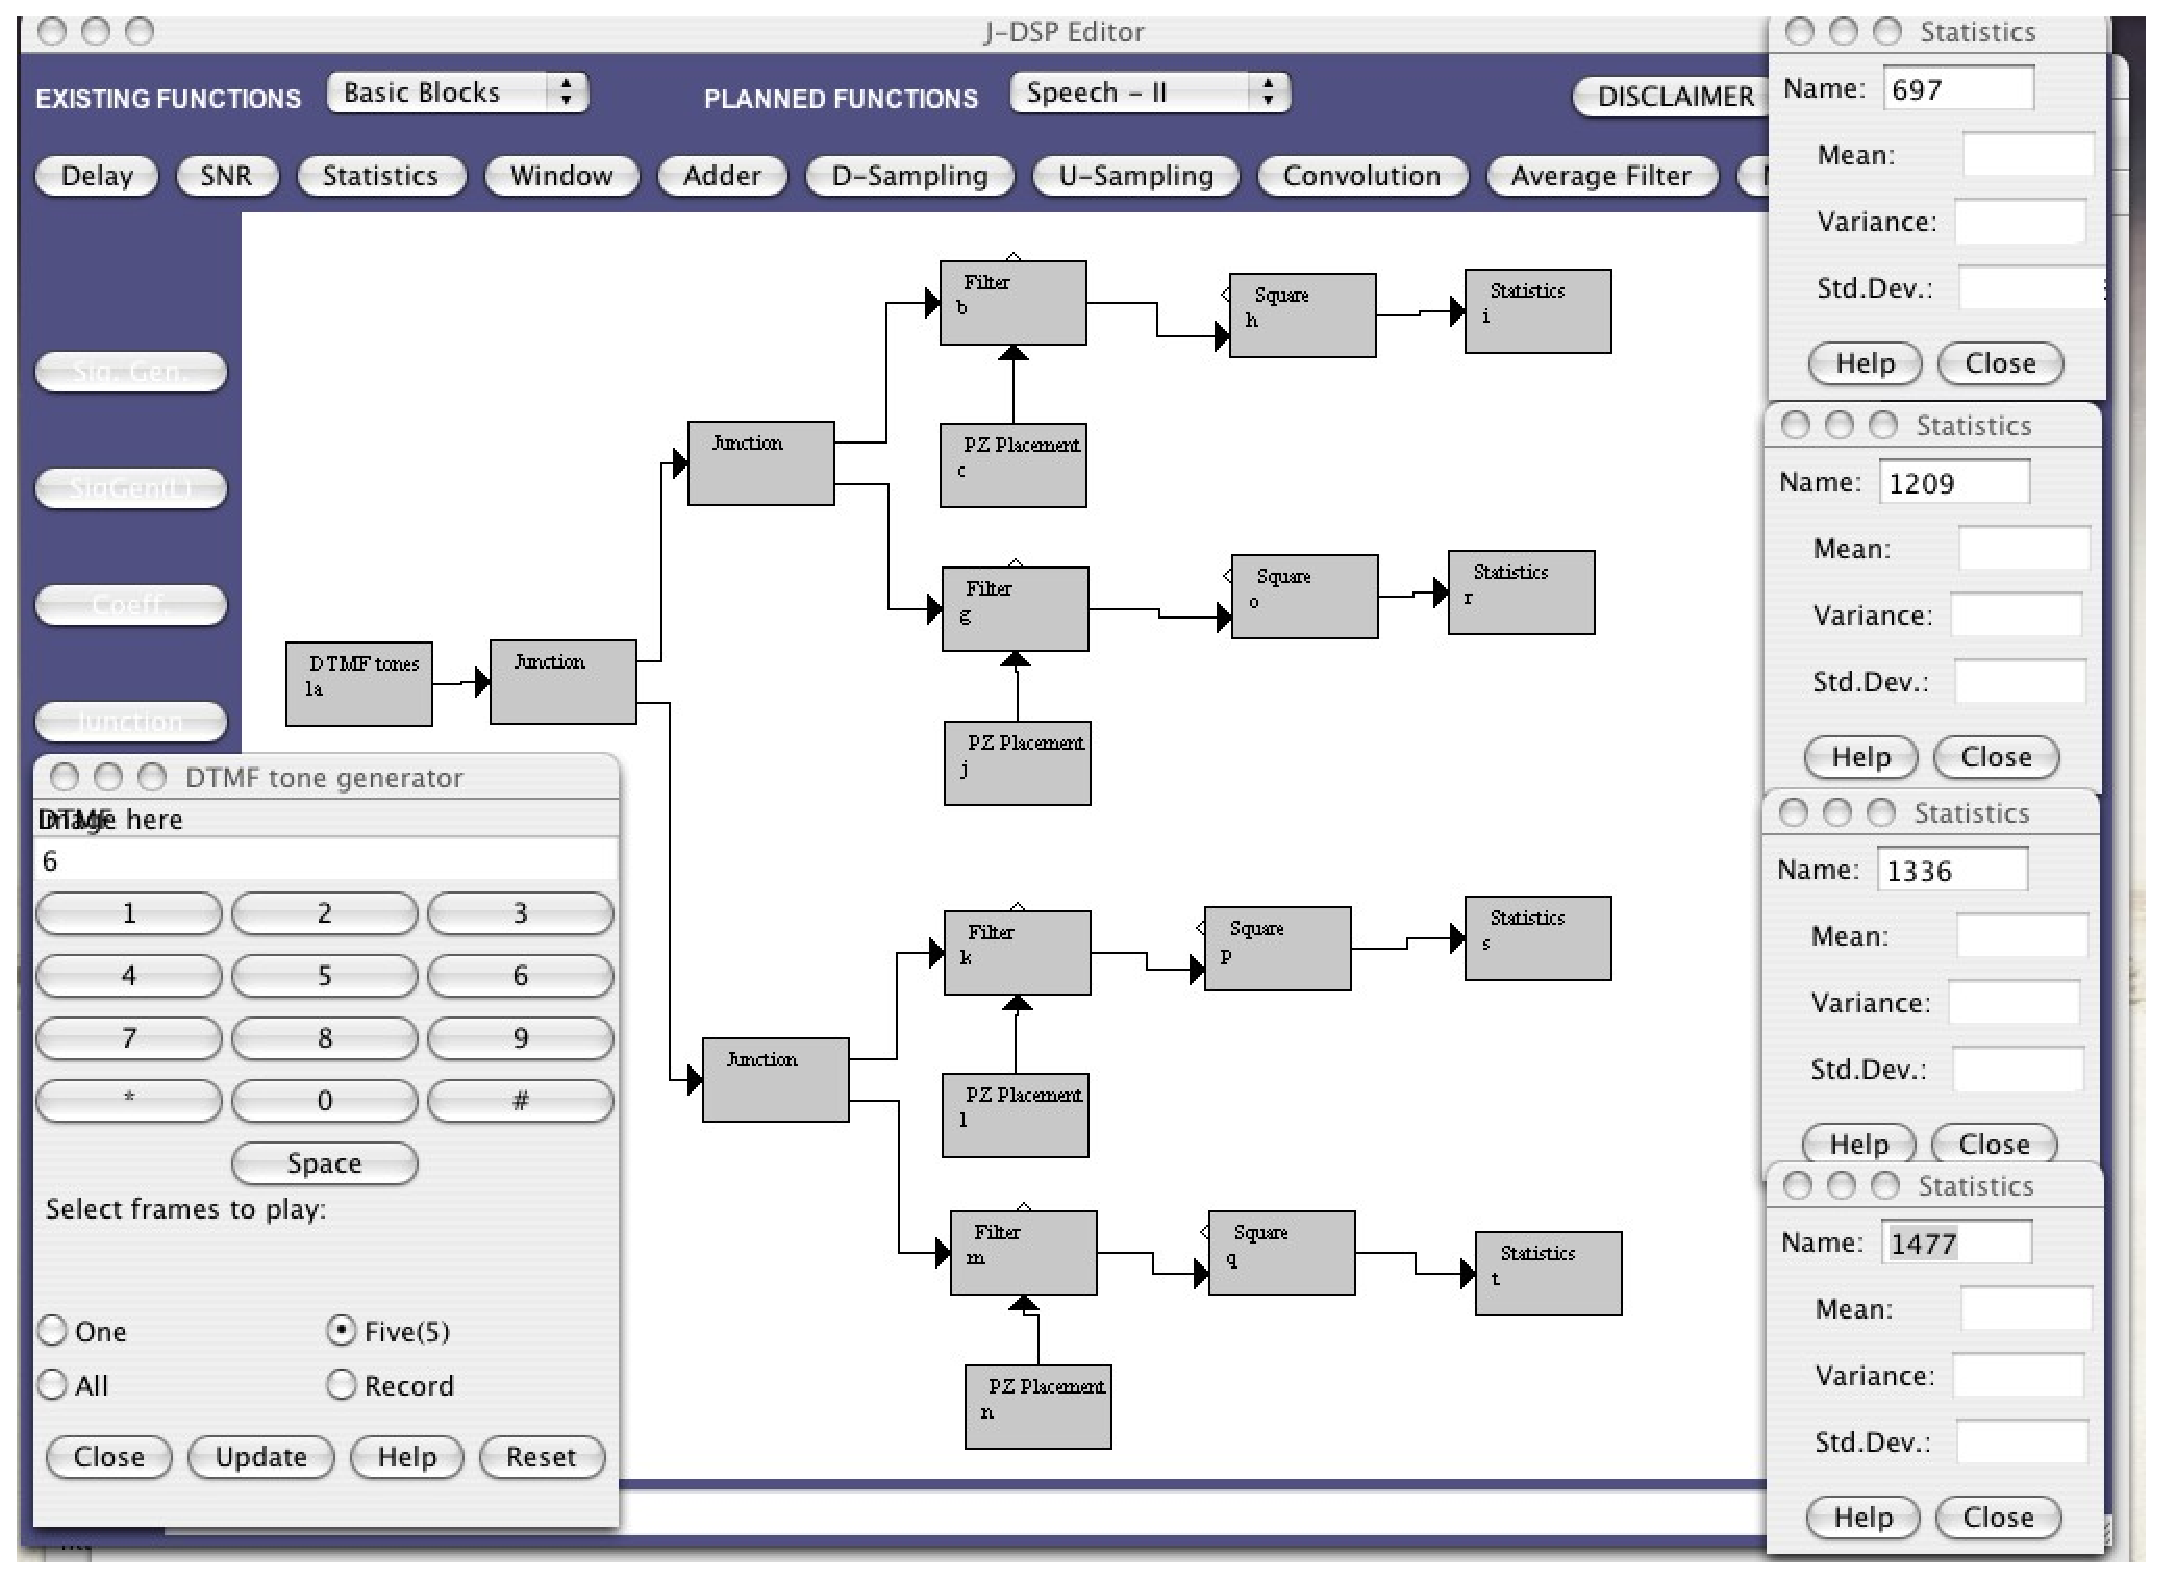
\includegraphics[width=6in]{lab7/screen}
  \end{center}
  \caption{Example filter bank layout.\label{fg:screen}}
\end{figure}

\paragraph{Step 2.4} Now we will assemble a filter bank. Your final layout 
should look something like Figure~\ref{fg:screen}. Pare down
your filter, etc. to the minimum set of blocks: \block{Filter},
\block{PZ Placement}, \block{Square}, and \block{Statistics}. Place four of these blocks down for
the four frequencies 697Hz, 1209Hz, 1336Hz, and 1477Hz; this will
allow us to recognize \button{1}, \button{2}, and \button{3}. Use
three \block{Junction}s to split the output of the \block{DTMF Tones}
block to send to four filters. Place the poles for each filter at the
same radius and the appropriate angles for each frequency (remember,
the \block{PZ Placement} block uses degrees for manual angle
entry). Name the \block{Statistics} blocks for the filters'
frequencies. Include a screen shot showing the output for
\block{DTMF Tones} button \button{2} in your report. What are the mean
squared values for each frequency for each of the \block{DTMF Tones}
buttons \button{1}, \button{2}, \button{3}, and \button{4}?  Would you
be able to use a simple pair of comparisons for each button to decode
which button was pressed? Why or why not?

% LocalWords:  WebQ MATLAB DSP

%&LaTeX

\section{Discrete Fourier Transform}

\subsection{Lab Background}
By the end of this lab you should have a firm understanding of how the
Discrete Fourier Transform (DFT) can be implemented exactly using the
Fast Fourier Transform (FFT). In addition you should be able to
identify common problems using the DFT to analyze signals. You will
also be familiar with a new tool, the spectrogram, that uses the DFT
as a function of time.

\subsection{Implementing the DFT}

% TODO: have them work with this block for a good implementation of the J-DSP
Recall that the DFT can be implemented directly from the analysis
equation. For a length $N$ signal $x[n]$,
\begin{align}
X[k]=\sum_{n=0}^{N-1}x[n]e^{-j \frac{2\pi}{N} nk} && \text{for $k = 0, 1, 2, \cdots N-1$}
\label{eq:dft}
\end{align}
The order of the implementation is $O(N)=N^2$. The following java code
can be used to implement the DFT in J-DSP. It is implemented without
any algorithmic speedup (i.e., it exactly mirrors equation
\ref{eq:dft}).  Example of raw DFT implementation:
	\begin{lstlisting}
public class MyFunction1
{
 public void myCode(double[]x1,double[]x2,double[]y1,double[]y2,
 	double[]b1,double[]a1,double[]b2,double[]a2,
 	double para1, double para2, double para3)
  {
  // x1, x2 - input at pin 0 and pin1
  // y1, y2 - output at pin 4 and pin5
  // raw DFT implementation
  double[] yImag;
  double[] yReal;
  yImag = new double[256];
  yReal = new double[256];
  double twoPiOverN = 2*Math.PI/256;
  for( int k = 0 ; k < 256 ; k++)
  {
    yReal[k] = 0;
    yImag[k] = 0;
    for( int n = 0 ; n < 256 ; n++)
    {
      yReal[k] += x1[n]*Math.cos(n*k*twoPiOverN);
      yImag[k] += -x1[n]*Math.sin(n*k*twoPiOverN);
    }
    y1[k] = Math.sqrt(yReal[k]*yReal[k]+yImag[k]*yImag[k]);
  }
 }
}
	\end{lstlisting}
Note that there is not a native support in java for complex numbers so
this arithmetic is written out explicitly in the code above. For
example, the equation $y=x\times e^{a}$ (where x is a real number)
must be explicitly written out using Euler's formula, and the real and
imaginary portions saved in separate variables, $y_{real}=x\times
\cos(a)$ and $y_{imag}=x\times \sin(a)$.

The FFT algorithm, on the other hand, can be used to reduce the
computation time of the DFT to $O(N)=N\log_2 N$ - a significant
speedup for even modest length signals.

\paragraph{Step 1.1}
Write some example code to multiply \emph{two} complex numbers,
$c=a\times b$. Remember to represent the variables by their real and
imaginary parts and save the real and imaginary parts in separate
variables.


\paragraph{Step 1.2} 
Use the \block{UserDefinedFun} block to implement the FFT using loops
(i.e., do not use recursion). The first part of this code performs a
bit reversal on the input array. Use the following code to perform the
bit reversal:
% make more explict, bit rev vrbl
\begin{lstlisting}
// bit reversal
int  index;
int  N = 256;
double[] reversedX1 = new double[256];
// need to shift 32 bit integer to make it an 8 bit reversal
int shift = (32-(int)Math.round(Math.log(N)/Math.log(2))); 
for( int n = 0 ; n < N ; n++){
  index = (Integer.reverse(n))>>>shift; //reverse and then shift down to 8 bit
  reversedX1[n] = x1[index]; 
}
\end{lstlisting}
Then iterate over the array $\log_2 N$ times! Remember to explicitly
carry out any complex arithmetic and take the magnitude of the output
array once the FFT is computed. Include a copy of the java code in
your report.

\paragraph{Step 1.3} 
Check your results in J-DSP using the \block{FFT} block. Your results
should be identical. Take the FFT of a sinusoid with a frequency of
$\pi/4$ radians per second using your FFT implementation and the
\block{FFT} block provided in J-DSP. Include a screenshot of the
output plots.



\subsection{Using the DFT}
% switch over to spectrogram example with DTMF - organize introduction
% for ease of use over multiple steps
\paragraph{Step 2.1} 
Create a sum of two sinusoids in J-DSP. Use the \block{FFT} block to
compute the FFT of the sum and then plot the FFT magnitude. Use a
frequency of $0.13\pi$ and $0.19\pi$ for the two sinusoids. Make sure
that the \option{pulsewidth} for each is set to 256. What does the
result look like? Does this make sense?


\paragraph{Step 2.2} At what index (or indices) does the FFT magnitude
reach its peak value(s)? What frequency (or frequencies) does this
correspond to?


\paragraph{Step 2.3} Change the frequencies of the sinusoids to
$0.13\pi$ and $0.14\pi$. Repeat steps 2.1 and 2.2. Do the results
still make sense?


\paragraph{Step 2.4} Replace the sum of two sinusoids in J-DSP with
the \block{DTMF} block under the \menu{Audio Effects} function
list. Press some of the keys in the \block{DTMF} block. Does the FFT
block show separate frequencies for each button?



\subsection{Spectrograms}
Comparing FFT graphs (as in the step 2.4) can be difficult to do. But
what if we could analyze the frequency content of a signal as a
function of time? That would make it easier to see differences in
frequency if a signal started changing (like a string of DTMF keys
pressed in turn). To do this we will need a new tool called the
\emph{Spectrogram}. The spectrogram is simply an algorithm for
computing the FFT of a signal at different times and plotting them as
a function of time. The spectrogram is computed in the following way:

\begin{enumerate}
\item A given signal is ``windowed.'' This means that we only take a
  certain number of points from the signal (for this example assume we
  are using a window of length 128 points). To start out, we take the
  first 128 points of the signal (points 0 through 127 of the input
  array).
\item Take the FFT of the window and save the it in a separate array.
\item Advance the window in time by a certain number of points. For
  instance we can advance the window by 64 points so that we now have
  a window of indices 64 through 191 from the input signal array.
\item Repeat steps 1-3, saving the FFT of each window, until there are
  no longer any points in the input array.
\item Form a 2-D matrix whose columns are the FFT magnitudes of each
  window (placed in chronological order). In this way, each row
  represents a certain frequency, each column represents a given
  instant in time, and the value of the matrix represents the
  magnitude of the FFT.
\end{enumerate}

The result is called a Spectrogram and is usually displayed as an RGB
image where blue represents small FFT magnitudes and red represents
larger FFT magnitudes (the \emph{Jet} colormap if you are familiar
with color visualizations). There is an art to choosing the correct
parameters of the spectrogram (i.e., window size, FFT size, how many
points to advance the FFT, etc.). Each parameter has tradeoffs for the
time and frequency resolution of the resulting spectrogram. For our
purposes here, we will not be concerned with these tradeoffs. Instead
we will be more interested in getting familiar with analysis using
spectrograms.

\paragraph{Step 3.1} Use the DTMF setup from step 2.4. Instead of
using the \block{FFT} block, use the \block{Spectrogram} block under
the \menu{Statistical DSP} function stack. Keep all parameters in the
\block{Spectrogram} set to the default. Set the \block{DTMF} block to
play five frames per key press. Press the number ``1.'' What does the
spectrogram look like? Are both frequencies present?


\paragraph{Step 3.2} Now set the \block{DTMF} block to
\option{Record}. Also set the \option{Resolution} parameter inside the
\block{Spectrogram} block to 4 or 8 (otherwise you may notice a lag
for updating the spectrogram - it can be considerably CPU intensive
for large input signals). The \option{Resolution} parameter controls
how many points the sliding window advances at each time step (larger
steps mean we take fewer FFTs). Press each key in the \block{DTMF}
block in turn. Does the spectrogram make it easier to judge the
frequency content of the keys? Include a screenshot for your report.

% LocalWords:  WebQ MATLAB DSP



\end{document}
% LocalWords:  MATLAB
